\documentclass[]{jsarticle}
\usepackage[dvipdfm]{graphicx}
\usepackage{here}
\usepackage{multicol}
\usepackage{comment}
\usepackage{moreverb}
\usepackage{ascmac,here,txfonts,txfonts}
\usepackage{color}
\usepackage{listings,jlisting}
\renewcommand{\lstlistingname}{リスト}
\lstset{
  breaklines = true,
  language=Java,
  basicstyle=\ttfamily\scriptsize,
  commentstyle={\itshape \color[cmyk]{1,0.4,1,0}},
  classoffset=1,
  keywordstyle={\bfseries \color[cmyk]{0,1,0,0}},
  frame=tRBl,
  framesep=5pt,
  showstringspaces=false,
  numbers=left,
  stepnumber=1,
  numberstyle=\tiny,
  tabsize=2,
}

\title{\LARGE {数値計算法 課題2(常微分方程式)}}
\author{\large {ME1507 芝田 将}}

\begin{document}

\maketitle

\section{ロジスティック方程式の初期値問題$y'(t)=(1-y)y ~~~ (0 \ge t \ge 2),~~ y(0)=0.1$に関する次の問(1-1)から(1-3)について以下の4つの各解法を使って答えよ。}

\begin{enumerate}
\item オイラー法
\item ホイン法
\item 4次のルンゲクッタ法
\item 2次アダムス・バッシュフォース法
\end{enumerate}

\subsection{$h=\Delta t = 0.1, 0.01$の場合に$y(2)$の近似値を求めよ。}

各解法で近似値を求めるプログラムをリスト\ref{kadai2-source}に示す。

\lstinputlisting[caption=課題2プログラム,label=kadai2-source]
{../src/kadai2.c}


実行結果を以下に示す。

\begin{lstlisting}[caption=実行結果,label=kadai2-result]
$ ./a.out
Please input a h value (0.1 or 0.01).
h > 0.1
オイラー法による解: 0.438414
ホイン法による解: 0.450483
ルンゲクッタ法による解: 0.450853
アダムスバッシュフォース法による解: 0.449984

$ ./a.out
Please input a h value (0.1 or 0.01).
h > 0.01
オイラー法による解: 0.449601
ホイン法による解: 0.450849
ルンゲクッタ法による解: 0.450853
アダムスバッシュフォース法による解: 0.450844
\end{lstlisting}


\subsection{結果を考察せよ}

微分解$y(2) = \frac{0.1 e^{2}}{0.1 (e^{2}-1)+1} = 0.450853...$との誤差はを表\ref{error}に示す。

\begin{table}[htbp]
\begin{center}
\caption{微分解との誤差}
\begin{tabular}{|c|c|c|} \hline
手法 & $h=0.1$の時の誤差率[\%] & $h=0.01$の時の誤差率[\%] \\ \hline
オイラー法 & 2.758992 & 0.277696 \\ \hline
ホイン法& 0.082067 & 0.000887 \\ \hline
4次のルンゲクッタ法 & 0.000000 & 0.000000 \\ \hline
2次アダムス・バッシュフォース法 & 0.192746 & 0.001996 \\ \hline
\end{tabular}
\label{error}
\end{center}
\end{table}

表\ref{error}より、4次のルンゲクッタ法、ホイン法、アダムスバッシュフォース法、オイラー法の順に精度が良い事が確認できる。
特に4次のルンゲクッタ法は小数点以下6桁まで0が並び誤差がほとんど無いことが確認できる。
ホイン法は2次、オイラー法は1次であるため、次数が大きければ大きいほど正確な値が計算できることが分かる。

\subsection{各解法による近似解を比較出来るようにグラフで表示せよ。}

各解法による近似解を比較するために、誤差率を図\ref{fig:error-comparison}に示す。

\begin{figure}
\centering
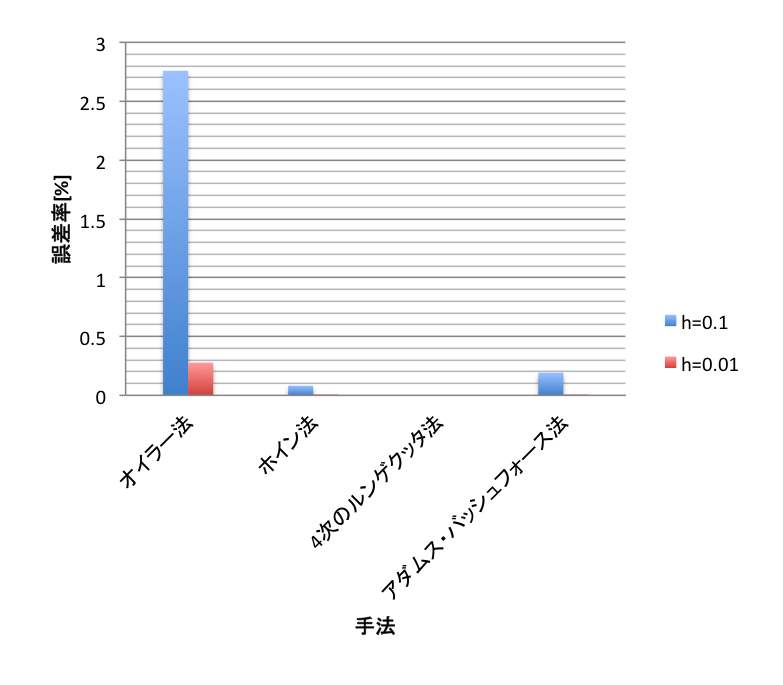
\includegraphics[width=100mm]{./img/error-comparison.eps}
\caption{各種法の誤差率の比較}
\label{fig:error-comparison}
\end{figure}

\section{2次アダムス・バッシュフォース法を導け}


\begin{eqnarray*}
\frac{dy}{dt} = f(t,y)\\
y(t_{0}) = y_{0}
\end{eqnarray*}

この微分方程式を解くには、$t_{n}$から$t_{n+1}$まで幅$h$で積分して、右辺の積分をラグランジュ補間式で近似する。
$k$次(過去の$k$個の点を使用)の場合には、次式のようになる。

\begin{eqnarray*}
y_{n+1} - y_{n} &=& \int_{t_{n}}^{t_{n+1}} f(t,y) dt\\
y_{n+1} &=& y_{i} + h(\beta_{1}^{k} f_{i} + \beta_{2}^{k} f_{i+1} + ... + \beta_{k}^{k} f_{i-k+1})
\end{eqnarray*}

各$f$に重み$\beta_{i-j+1}^{k}$を書けて総和を取ることで精度が向上している。
上式より2次のアダムスバッシュフォース法では、以下のとおりになる。

\begin{eqnarray*}
y_{n+1} = y_{i} + h(\frac{3}{2} f_{i} - \frac{1}{2} f_{i-1})
\end{eqnarray*}


\section{2次のアダムス・モルトン法(台形法)が2次の方法であることを示せ}

アダムス・モルトン法は、$x_{i}$から$x_{i+1}$の$f$の値を$f_{i+1}, f_{i}, ... , f_{i-k+2}$までの$k$個の値を内挿して求める。

\begin{eqnarray*}
y_{n+1} = y_{i} + h(\gamma ^{k}_{1} f_{i+1} + \gamma ^{k}2 f_{i} + ... + \gamma ^{k}_{k} f_{i-k+2})
\end{eqnarray*}

よって2次の場合は、次式のようになる。

\begin{eqnarray*}
y_{n+1} = y_{i} + h(\frac{1}{2} f_{i+1} + \frac{1}{2} f_{i})
\end{eqnarray*}

これは2次のアダムスバッシュフォース法と同じであることから、台形法であるアダムスモルトン法も2次の方法であることが確認できる。


\section{P110 第5章 演習問題7を解け}

\begin{eqnarray*}
\ddot{y} + 2k\dot{y} + \omega ^{2} y &=& 0 \\
y(0) &=& 1 \\
\dot{y}(0) &=& 1
\end{eqnarray*}

1階微分方程式に変形。

\begin{eqnarray*}
\dot{y}_{1} &=& y_{2}\\
\dot{y}_{2} &=& - \omega ^{2} y_{1} - 2k y_{2}\\
y_{1}(0) &=& 1\\
y_{2}(0) &=& 0 
\end{eqnarray*}

差分法を用いて一階微分方程式と二階微分方程式の近似式を求める。

\begin{eqnarray*}
\frac{1}{\Delta t}(Y^{1}_{j+1} - Y^{1}_{j}) &=& f_{1}(t_{j}, Y_{j}^{1}, Y_{j}^{2})\\
\frac{1}{\Delta t}(Y^{2}_{j+1} - Y^{2}_{j}) &=& f_{2}(t_{j}, Y_{j}^{1}, Y_{j}^{2})\\
Y^{1}_{0} &=& 1\\
y^{2}_{0} &=& 0 
\end{eqnarray*}

常識に一回微分方程式を代入。

\begin{eqnarray*}
Y^{1}_{j+1} &=& Y^{1}_{j} + \Delta t Y_{j}^{1}\\
Y^{2}_{j+1} &=& -\omega^{2} \Delta t Y_{j}^{1} + (1-2k\Delta t)Y_{j}^{2}\\
Y_{0}^{1} &=& 1\\
Y_{0}^{2} &=& 0
\end{eqnarray*}

これを解くと、$Y_{j}^{1}$は

\begin{eqnarray*}
Y_{j}^{1} = \frac{9}{8} ( 1-10 \Delta t)^{j} - \frac{1}{8} ( 1- 90\Delta t)^{j} 
\end{eqnarray*}

となる。$\Delta t \to 0$の極限では$j\Delta t = t$とすると、

\begin{eqnarray*}
(1-10 \Delta t)^{j} \to exp(-10t)\\
(1-90 \Delta t)^{j} \to exp(-90t)\\
y(t) = \frac{9}{8} exp(-10t) - \frac{1}{8} exp (-90t)
\end{eqnarray*}

tが大きくなると急速に0に近づく。差分解の項が0に近づくためには、$|1 - 10 \Delta t| < 1$かつ$|1 - 90 \Delta t| < 1$、つまり$\Delta t < \frac{1}{90}$に設定すれば、差分解は滑らかに減衰する。


\end{document}